\documentclass[11pt]{article}
%Gummi|061|=)


%\begin{figure}[ht]
%\centering
%\subfigure[Caption of subfigure 1]{
%    \rule{4cm}{3cm}
%    \label{fig:subfig1}
%}
%\subfigure[Caption of subfigure 2]{
%    \rule{4cm}{3cm}
%    \label{fig:subfig2}
%}
%\subfigure[Caption of subfigure 3]{
%    \rule{4cm}{3cm}
%    \label{fig:subfig3}
%}
%\caption[Optional caption for list of figures]{Caption of subfigures \subref{fig:subfig1}, \subref{fig:subfig2} and \subref{fig:subfig3}}
%\label{fig:subfigureExample}
%\end{figure}


\title{\textbf{Search-based Planning for Dual-arm Manipulation with Upright Orientation Constraints}}
\author{Review by Igor Bogoslavskyi\\
		Humanoid Robots Seminar\\Albert Ludwigs Universitat Freiburg\\
Email: bogoslai@informatik.uni-freiburg.de}
\date{}

\usepackage[tight,footnotesize]{subfigure}
\usepackage{graphicx}
\usepackage{subfigure}
\DeclareGraphicsExtensions{.pdf,.png,.jpg}

\hyphenation{op-tical net-works semi-conduc-tor res-pect constraint}

\begin{document}

\maketitle

\begin{abstract}
%\boldmath
This paper presents an algorithm for dual-arm manipulation with upright orientation constraints. Dual-arm manipulation is essential for dealing with large objects as they are harder to grasp and manipulate using single arm. The upright constraint on the grasped objects is also widely used in human indoor environments, e.g. when manipulating a tray with food or liquids.\\
The algorithm presented in this paper produces an optimal and consistent solution to the planning of dual-arm motions problem so that it is guaranteed that robot would choose the same sequence of motions given the same start and goal configurations. These motions come with guarantees on completeness and bounds on the suboptimality with respect to the graph that encodes the planning problem.\\
This is achieved by constructing a graph in task space and using A* like seach techniques to find optimal path from start configuration to goal configuration.\\
Overall, the algorithm provided in this paper is capable of planning consistent optimal dual-arm motions in cluttered environments, often within one second.

\end{abstract}

\begin{figure}[htb]
\centering
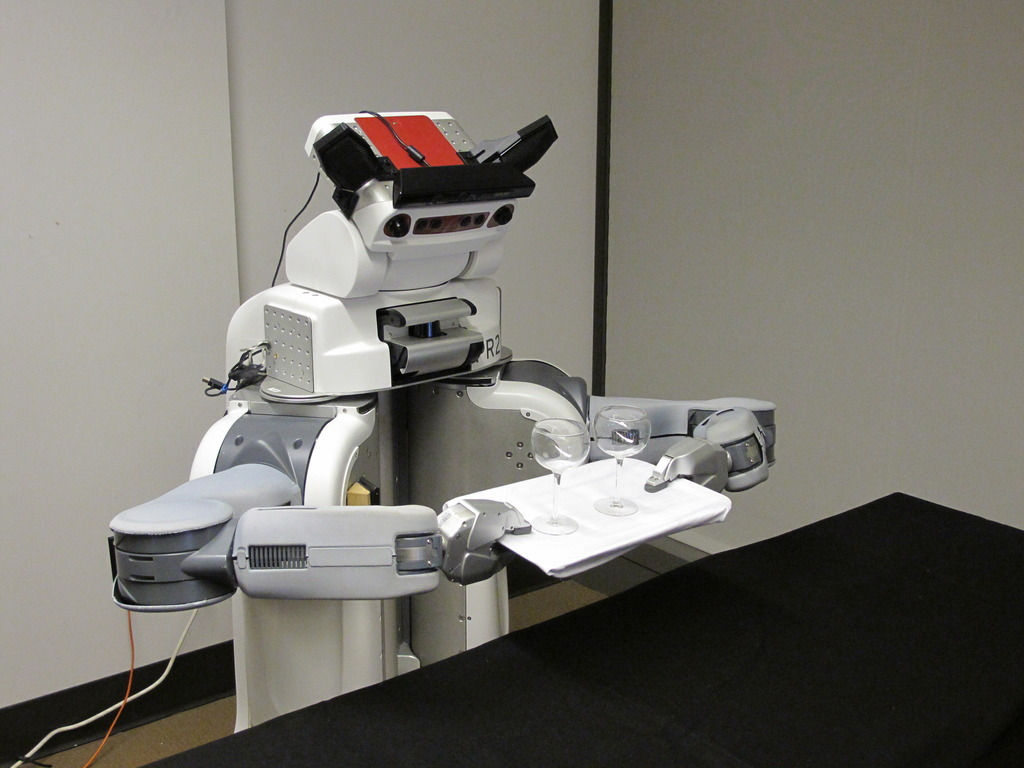
\includegraphics[width=0.7\textwidth]{dual-000.jpg}
\caption{The PR2 robot holding a tray with glasses}
\label{fig:PR2 with glasses}
\end{figure}



\section{Introduction and Related Work}
% no \IEEEPARstart
This report is  a review of the article \emph{Search-based Planning for Dual-arm Manipulation with Upright Orientation Constraints} by \emph{Benjamin Cohen, Sachin Chitta} and \emph{Maxim Likhachev}, published at \emph{IEEE Int. Conference on Robotics and Automation} in 2012, see [24].\\
In human environments it is sometimes hard or even impossible to deal with an object using only one hand. For example, carying any big objects such as big boxes or objects that require correct orientation is space such as trays with glasses etc. is much easier with the use of both hands instead of just using one. This is why these tasks are often performed with usage of both hands by human. This is the motivation for performing such tasks with two arms by a general mobile robot.\\


As was mentioned before, sometimes it is necessary to hold and carry objects with constraints on their orientation. For example, carying a tray with food or glasses requires naturally an upright orientation constraint at each moment of the movement. In real life these tasks are usually performed by humans in cluttered environments e.g. moving a tray through an environment full of obstacles. These tasks involve fast and efficient planning of actions, while retaining the upright orientation constraint. This is exactly what is addressed in this paper.\\
The robot that was used for this task is the PR2 robot. In Figure 1 it is shown holding a tray with two wine glasses on it. For this task the robot has to maintain the upright orientation of the tray throughout the sequence of arm motions. Navigating in cluttered environments with a tray is a hard task, that involves many different parts such as planning the collision-free apth through the environment while preserving the upright orientation constraint of the tray. The authors of the paper focus only on the dual-arm manipulations part.\\
Motion planning for dual-arm manipulations is addressed as a graph search problem in this paper. The graph is constructed in action space and heuristic search such as A* [8] and its variants is used to find the optimal sollution to the problem.\\
In recent years manipulating objects in human environments gained a lot of interest ([19], [18], [7], [1], [11], [2], [22]). The works [4],[5] and [6] show successfull usage of A*-like search algorithms on graphs with correspondence to motion planning including single arm manipulations and other mobile manipulation tasks. These algorithms have advantages such as good cost optimmization and strong theoretical guarantees on completeness and optimality or bounds on the sub-optimality of the sollution [17]. Another benefit of graph-based techniques is their consintensy. That makes the robot behave predictably given the same start and goal poses which is very important in human environments as people are able to predict the robot's actions better.\\
On the other hand, the gurantees of optimality as well as consistensy are with respect to the graph which is used to represent the planning problem, so they are discretization of state and action space dependent.\\
However the A*-like algorithms were never used for dual-arm manipulations before. Recently, as interest in dual-arm manipulations has rised, a couple of dual-arm platforms became available, e.g. the robot used in this paper - PR2 [3] (Fig. 1), Intel HERB Personal Robot [22], ARMAR III [23] and Justin [2]. Dual-Arm manipulation was already used for tasks like cart-pushing [21], towel folding [16] and the manipulation of small kitchen objects [23]. Usually, unlike the approach chosen by the authors of this paper, randomized motion planners were chosen to perform on above mentioned tasks. For example, in [23], randomized motion planners were used for planning re-grasping actions and dual-arm motion plans for a humanoid robot with two arms. Impressive results for combined grasping and motion planning were achieved by interleaving the efficient computation of inverse kinematics using a pre-computed reachability map with the motion planning itself. In [10], an assembly task was executed with two arms using combined task and motion planning. Online manipulation planning for objects moving on a conveyer belt was carried out in [14] for two 2-DOF arms. In [12], one of the first approaches to planning for dual-arm manipulation was presented using a randomized planner. Multi-arm manipulation planning, including the planning of transfer paths and grasp and ungrasp motions for manipulating an object using multiple arms was presented in [13]. The results of this approach were demonstrated on a simulated system manipulating a simple object using 3 arms.\\
Randomized planners for dual-arm manipulation tasks are a popular choise popular because of their speed and ease of implementation. However, plans generated by such planners require frequent post-processing, e.g. using a short- cutting approach [9], before they can be executed on a robot. In addition, due to the random nature of the planners, the generated paths are also inconsistent across runs, i.e. paths planned for the same environment for similar start and goal positions are likely to be very different. Search-based planning addresses this issue providing consistency between runs and reasonable cost minimization.\\
The authors of this paper present a graph-based A* search approach for dual-arm manipulation that is based on two key components: the representation of the state space and a novel heuristic. 
The representation of the state space is chosen so that it reduces the dimentionality of the problem and thus makes it easier to ba handeled via search-based techniques. It also helps dealing with discretization artifacts that authors of the paper have experienced in their former work [6].
The heuristic function is chosen in the way that it exploits the upright orientation constraint of the object. This provides additional information for motions in a cluttered environments.\\
This paper will focus mostly on these two concepts.

\section{The PR2 Robot REWRIGHT}
The hardware platform that was used for experiments by the authors of the paper was the PR2 mobile manipulation robot (Fig. 1). The PR2 robot is a two-armed robot with an omni-directional base and a variety of sensors mounted on a sensor head. Each arm has 7 degrees of freedom and thus has a redundant degree of freedom. In this paper, the redundancy is exploited by developing a custom inverse kinematics solution for the arm that is parameterized by one of the joint angles. The joint angle we choose is the upper arm roll joint shown in Fig. 3(b). The joint limits on the robot’s joints are also taken into account by the kinematics solver. Thus, given the end-effector pose and a value for the free parameter, we can deterministically compute the corresponding inverse kinematics solution for this pose. In general, because of joint limits, we tend to find only a single solution (if it exists) for a given end-effector pose and free angle parameter. If a solution does not exist, it is possible to step through the full range of motion of the redundant joint to search for an inverse kinematics solution.

\section{Motion Planning Algorithm (under construction)}
The morion plasnnin algorithms described in this paper is based on constructing and serching a motion-primitive based graph [5] using pre-defined and runtime-generated motion primitives. The graph search is supposed to find a path from start configuration of the robot to its goal configuration (location and orientation).\\
The algorithm consists of these four parts:\\
 - Graph constuction;\\
 - Cost function;\\
 - Heuristic;\\
 - Search;

\end{document}
